\documentclass[a4paper,12pt]{article}
\usepackage[utf8]{inputenc}
\usepackage[ngerman]{babel}
\usepackage{graphicx}
\usepackage[a4paper,margin=2.5cm]{geometry}
\usepackage{parskip}
\usepackage{helvet}
\renewcommand{\familydefault}{\sfdefault} % Serifenlose Schrift

\begin{document}
\thispagestyle{empty} % Keine Kopf-/Fußzeile

\vspace*{1cm}

% Titel oben
\begin{center}
  {\Huge \textbf{Bewerbung}}\\[0.3cm]
  {\large um einen Minijob im Homeoffice}\\[0.2cm]
  {\large im Bereich \textbf{Datenerfassung und digitale Büroarbeit}}
\end{center}

\vspace{1.8cm}

% Bewerbungsbild zentriert
\begin{center}
  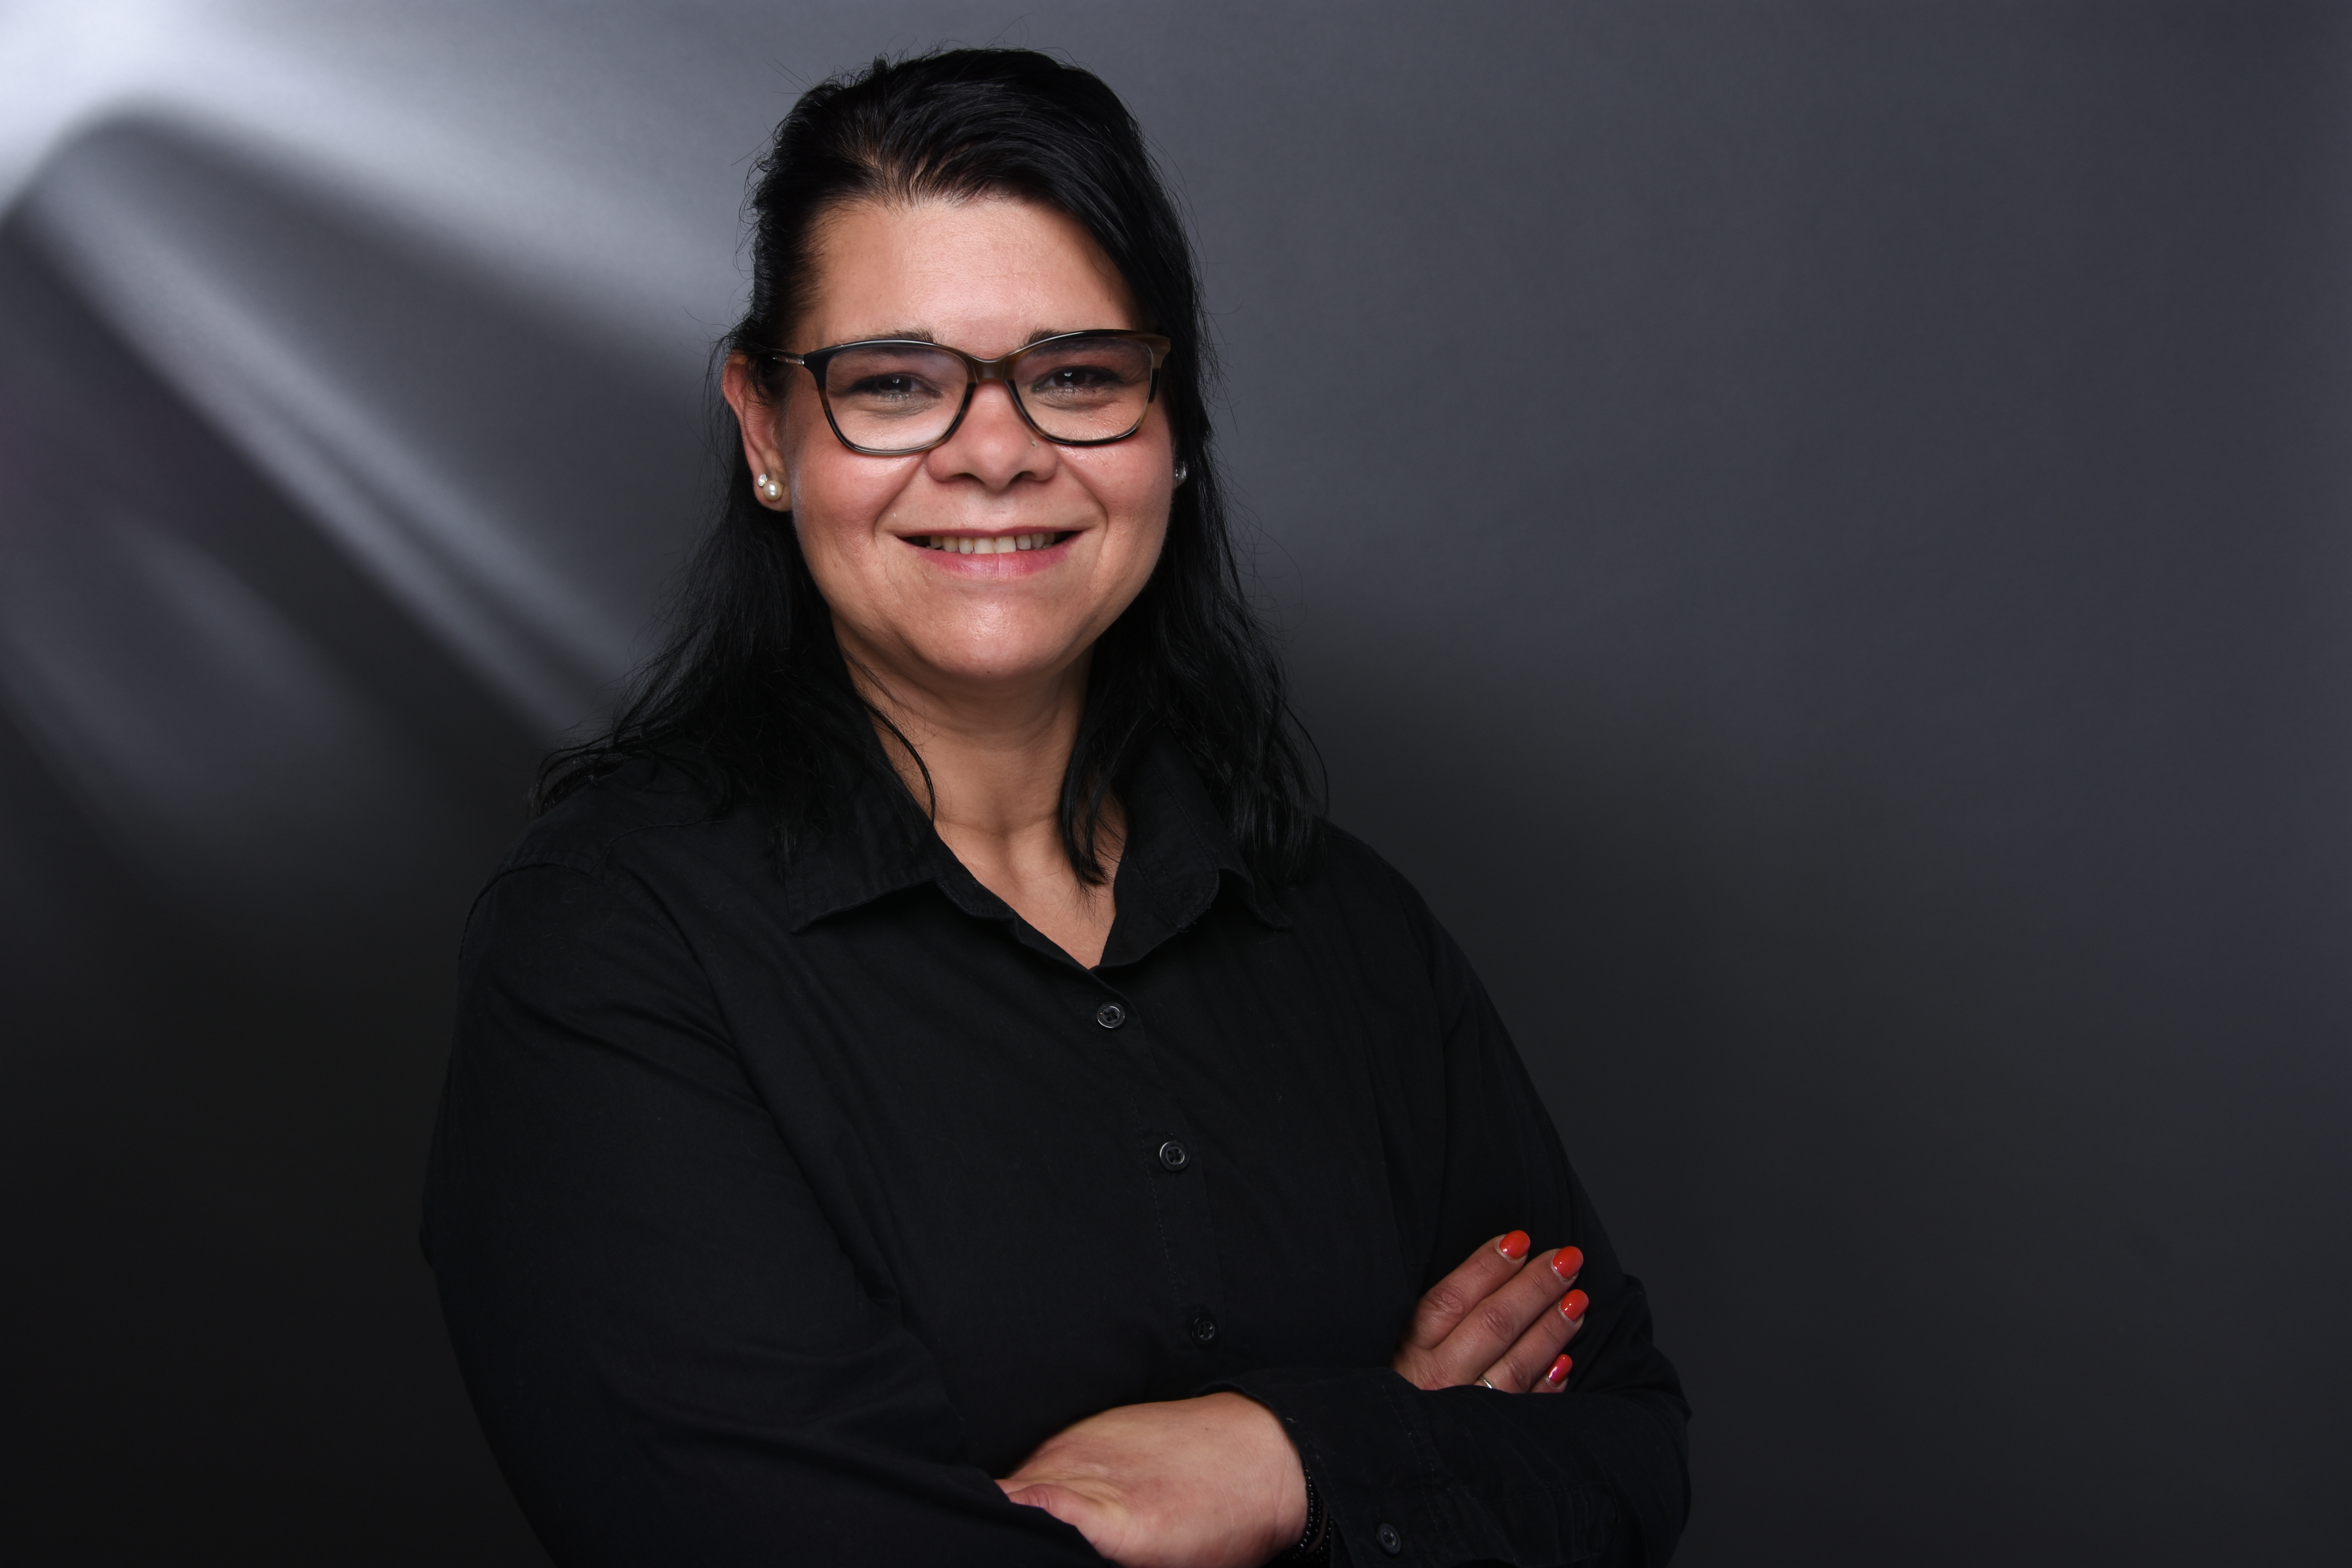
\includegraphics[width=6.5cm]{img/Bewerbungsfoto.jpg} % ← Pfad ggf. anpassen
\end{center}

\vfill

% Persönliche Angaben unten
\begin{center}
  \textbf{Eveline Renges} \\
  Schwalbenhälde 26\\
  74354 Besigheim \\
  Telefon: +49 176 478 56446\\
  E-Mail: evelinerenges@proton.me \\
  % GitHub: \texttt{github.com/patrick-renges} \\
  % LinkedIn: \texttt{linkedin.com/in/patrick-renges}
\end{center}

\vspace{1cm}

% Datum
\begin{center}
  \today
\end{center}

\end{document}
